
\subsection{Translation and Ribosomal Synthesis as a Growth-Rate Limiting Step}
Thus far, the general back-of-the-envelope estimates have been reasonably
successful in explaining what sets the scale of absolute protein copy number. A
recurring theme that has arisen is the ability of cells to parallelize their
biosynthesis tasks. For example, while DNA replication speed-limit is $\approx$
40 minutes to replicate a genome, cells can divide faster than this by
initiating more than one round of replication per doubling. The process of
protein synthesis overall  doesn't appear to be rate-limiting, since for
example, cells are able to induce the  expression of additional enzymes to grow
on alternative carbon sources.  However, as we will see, the synthesis of ribosomal
proteins presents a special case where parallelization is not possible
(\FIG{ribosome_limit}(A)). Thus, it is plausible that translation may be a key
factor in determining the cellular growth rate.

% In many cases, these estimates can be adapted to consider a continuum of
% growth rates in lieu of our single 5000 s point estimate, the details of which are
% described in the Supplemental Information.
% growth on different carbon sources
% is achieved by inducing the expression of
% resulted in the induced
% expression of particular transporters, often producing more
% than needed to acquire enough carbon to build new cell mass (\FIG{carbon_transport}(B)). In
% examining replication of the DNA, we described how cells can replicate multiple
% copies of the chromosome at any given time, permitting growth rates faster than
% the limit at which the chromosome can be faithfully replicated.
% As another related example, we showed how increasing the gene dosage of the rRNA operons is
% necessary to produce enough rRNA to form functional ribosomes.

%
% Understanding the allocation of resources and large-scale structure of bacterial
% proteome has been an area of intense quantitative study over the last decade by Hwa and others
% \citep{scott2010, hui2015}. From the perspective of limiting growth, our
% earlier estimate of rRNA highlighted the necessity for multiple copies of
% rRNA genes in order to make enough rRNA. For \textit{E. coli}'s fastest
% growth rates at 2 hr$^{-1}$, the additional demand for rRNA is further
% supported by parallelized DNA replication and increased rRNA gene dosage.
% This suggests the possibility that synthesis of ribosomes might become rate
% limiting.

To gain some intuition into how translation can set the speed of
bacterial growth, we again consider the total number of peptide bonds that must
be synthesized, which we denote as $N_\text{AA}$. With cells growing exponentially in time
\citep{godin2010}, we can compute the number of amino acids to be polymerized as
\begin{equation}
    N_\text{AA} \lambda = r_t R,
\end{equation} where
$\lambda$ is the cell growth rate in s$^{-1}$, $r_t$ is the maximum translation
rate in AA$\cdot$s$^{-1}$, and $R$ is the average ribosome copy number per
cell. Knowing the number of peptide bonds to be formed permits us to compute the
translation-limited growth rate as
\begin{equation}
\lambda_\text{translation-limited} = \frac{r_t R}{N_\text{AA}}.
\end{equation}

Alternatively, since $N_{AA}$ is related to the total protein mass through the
molecular weight of each protein, we can also consider the growth rate in terms
of the fraction of the total proteome mass dedicated to ribosomal proteins. By
making the approximation that an average amino acid has a molecular weight of
110 Da (BNID: 104877, \cite{milo2010}), the total protein mass $m_{\textrm{protein}}$ is related to
$N_{AA}$ by $(m_{\textrm{protein}}/\text{110 Da}) \times N_A$, where $N_A$ is Avogadro's number.
Similarly, $R$ is related to the ribosomal protein mass by $R \approx
(m_R/\text{800 Da}) \times N_A$, where 800 Da reflects the summed molecular weight
of all ribosomal subunits.  This allows us to approximate  $R / N_\text{AA}
\approx \Phi_R / L_R$,  where $\Phi_R$ is the ribosomal mass fraction $m_{\textrm{protein}}/m_R$,
and $L_R$ the ratio of 800 kDa / 110 Da per amino acid or, alternatively, the
total length in amino acids that make up a ribosome. The translation-limited
growth rate can then be written in the form
\begin{equation}
\lambda_{\textrm{translation-limited}} \approx \frac{r_t}{L_R}  \Phi_R.
\label{eq:translation_limit_growth_rate}
\end{equation}
This is plotted as a function of ribosomal fraction $\Phi_R$ in
\FIG{ribosome_limit}(B), where we take $L_R$ = 7459 AA, corresponding to the
length in amino acids for all ribosomal subunits of the 50S and 30S complex
(BNID: 101175, \citep{milo2010}).

The growth rate defined by \EQ{translation_limit_growth_rate} reflects
mass-balance under steady-state growth and has long provided a rationalization
of the apparent linear increase in \textit{E. coli}'s ribosomal content as a
function of growth rate \citep{Goldberger1979, scott2010}. Here we see that
there will be a maximum rate when $\Phi_R$ = 1, which for a translation rate of
17 amino acids per second, gives us $\lambda \approx 8 \,\text{hr}^{-1}$, or a
doubling time just under 6 minutes (\FIG{ribosome_limit}(B), dashed line).
Interestingly, this limit is independent of the absolute number of ribosomes and
is simply given by the time to translate an entire ribosome, $L_R/ r_t$. As
shown in \FIG{ribosome_limit}(A), we can reconcile this with the observation
that in order to double the average number of ribosomes, each ribosome must
produce a second ribosome and this process cannot be parallelized. Unless
protein synthesis can increase, or cells can trim their total ribosomal protein
mass, this must represent an absolute speed limit for cell doubling.

\begin{figure}
  \begin{fullwidth}
        \centering{
            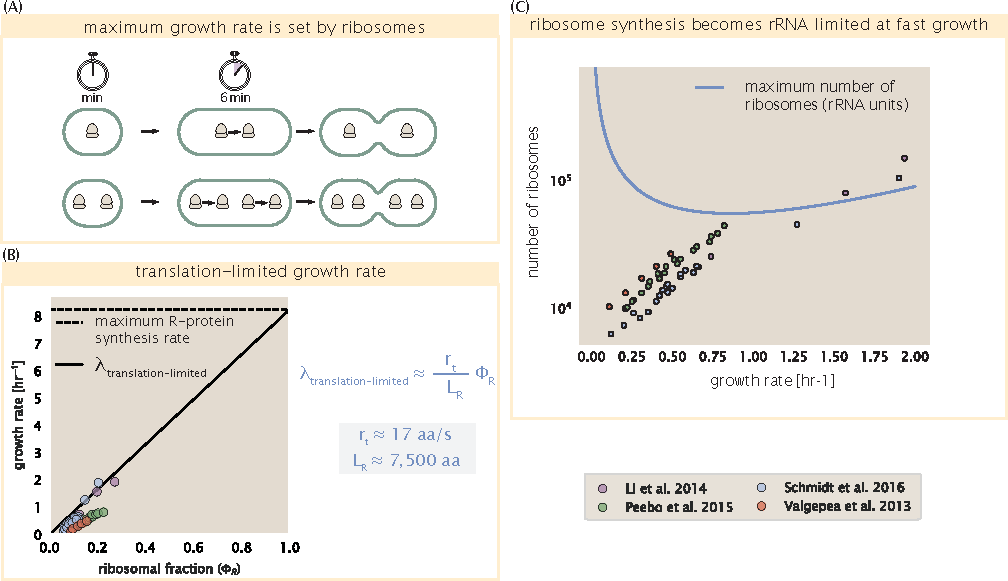
\includegraphics{main_figs/fig7_ribosome_growth_limit_2.pdf}
            \caption{\textbf{Translation-limited growth rate.}  (A) An inherent
            maximum growth rate is set by the ttime to synthesize all ribosomal
            subunits. This growth rate is given by $r_t/ L_R$, where $r_t$ is
            the elongation rate and $L_R$ is the total number of amino acids
            that make up the entire ribosomal complex. This rate is independent
            of the number of ribosomes; instead limited serial requirement for
            each ribosome to double itself. (B) Here we consider the
            translation-limited growth as a function of ribosomal fraction, as
            defined in Equation \ref{eq:translation_limit_growth_rate}. The
            solid line is calculated for an elongation rate of 17 aa per second.
            The dashed line corresponds to the maximum rate of ribosomal protein
            (R-protein) synthesis considered in part (A). [inset needed to show
            smaller region where data is.] (C) Maximum number of
            rRNA units that can be synthesized as as a function of growth rate.
            Solid curve corresponds to the rRNA copy number is calculated by
            multipyling the number of rRNA operons by the estimated number of
            $\langle\text{\# ori}\rangle$ at each growth rate. The quantity
            $\langle\text{\# ori}\rangle$ was calculated using Equation 4 and
            the measurements from \cite{si2017} that are plotted in
            \FIG{translation_ecoli_partA}(A). The dashed line shows the maximal
            number of functional rRNA units produced from a single chromosomal
            initiation per cell cycle. }
        \label{fig:ribosome_limit}
        }
  \end{fullwidth}
\end{figure}

Earlier, we considered rRNA synthesis (see Section \textit{\bf RNA Synthesis}),
finding that, when the rRNA operons are maximally loaded with RNA polymerase,
the cell can produce $\approx$ 1 functional rRNA unit per second per operon. In
\FIG{ribosome_limit}(C), we show the maximum number of ribosomes that could be
made as a function of growth rate given this rRNA production rule-of-thumb.
While each \textit{E. coli} genome has 7 copies of the rRNA operon (BNID:
107866, \cite{milo2010}), parallelization of DNA synthesis by firing multiple
rounds of replication at a time can drastically the effective number of rRNA
operons. The blue curve in \FIG{ribosome_limit}(C), we assume that the effective
number of rRNA operons increases in proportion to the number of origins of
replication $\langle\text{\# ori}\rangle$ (solid blue line; with the calculation
of $\langle\text{\# ori}\rangle$ described in the next section). Although we
expect this value to drastically overestimate rRNA abundance at slower growth
rates ($\lambda < 0.5\, \text{hr}^{-1}$), it provides a useful reference when
considered along with the proteomic measurements that are also plotted. For
growth rates above about 1 hr$^{-1}$, we find that cells will need to transcribe
rRNA near their maximal rate.  The dashed blue curve in \FIG{ribosome_limit}(C)
shows the maximal number of functional rRNA units that could be synthesized from
a single genome (ignoring the chromosome replication speed limit of $\approx$ 40
minutes per genome). The convergence between the maximum rRNA production with
parallelization and the experimentally measured ribosome copy number (points in
\FIG{ribosome_limit}(C)), suggests rRNA synthesis may begin to present a
bottleneck in cell division at the fastest growth rates. While this strain of
\textit{E. coli} is rarely reported to grow faster than 2 hr$^{-1}$, other
bacteria with more copies of rRNA genes have been found that surpass this growth
rate \citep{bremer2008,roller2016}.
